\documentclass[14pt]{article}
\usepackage[margin=1in]{geometry}
\usepackage{graphicx}
\usepackage{mathcomp}
\title{201 Lab 2\\Spreadsheets and Plots}
\author{Andreas Smit\\30065542}

\begin{document}
    \maketitle
    \begin{table}[h]
        \caption{Constants and Given Data}
        \centering
            \begin{tabular}{|c|c|}
                \hline
                Barametric Pressure (kPa) & 80\\
                \hline
                Temperature (\textcelsius) & 4\\
                \hline
                mass (g) & 3.43\\
                \hline
                Molar mass (g/mol) & 70\\
                \hline
                Moles (mol)& 0.049\\
                \hline
            \end{tabular}
    \end{table}
    \begin{table}[h]
        \caption{Lab Data}
        \centering
            \begin{tabular}{|c|c|c|c|c|c|c|}
                \hline
                Run \#&$P_{gauge}$ &$P_{abs}$& $V_{pr}$ &$\Delta V_p$ &$V_f$ &$V_m$\\
                Units&(kPag)&(kPaa)&(cm$^3$)&(cm$^3$)&(cm$^3$)&(cm$^3$/mol)\\
                \hline
                Start&1840&1920&140&&70&1428.57142857143\\
                2&2180&2260&145&5&65&1326.5306122449\\
                3&2330&2410&150&10&60&1224.48979591837\\
                4&2450&2530&155&15&55&1122.44897959184\\
                5&2570&2650&160&20&50&1020.40816326531\\
                6&2730&2810&165&25&45&918.367346938775\\
                7&2850&2930&170&30&40&816.326530612245\\
                8&2860&2940&170.88&30.88&39.12&798.367346938776\\
                9&2840&2920&175&35&35&714.285714285714\\
                10&2870&2950&180&40&30&612.244897959184\\
                11&2880&2960&185&45&25&510.204081632653\\
                12&2870&2950&190&50&20&408.163265306122\\
                13&2880&2960&195&55&15&306.122448979592\\
                14&2870&2950&200&60&10&204.081632653061\\
                15&2870&2950&205&65&5&102.040816326531\\
                16&2870&2950&206.56&66.56&3.44&70.204081632653\\
                17&5380&5460&208.58&68.58&1.42&28.9795918367344\\
                18&5740&5820&208.73&68.73&1.27&25.918367346939\\
                \hline
            \end{tabular}
    \end{table}
    \begin{figure}[h]
        \vspace{-80pt}
        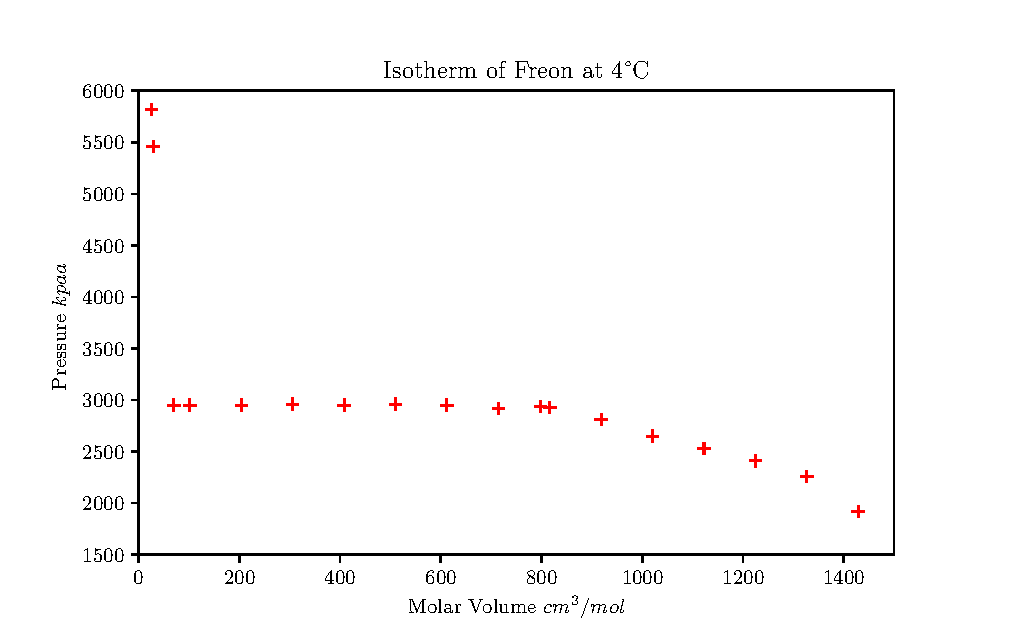
\includegraphics[width=\columnwidth]{fig1.eps}
    \end{figure}
    \begin{table}[h]
        \caption{Class Experimental Data}
        \centering
            \begin{tabular}{|c|c|c|c|c|}
                \hline
                Group Number & Temperature& Pressure & BUBBLE POINT & DEW POINT\\
                & \textcelsius & kPa& Specific Volume ($m^3/kg$)&Specific Volume ($m^3/kg$)\\
                \hline
                1&0&4.743&0.00189&0.09653\\
                2&16&7.515&0.001975&0.06149\\
                3&32&11.33&0.002078&0.04048\\
                4&48&16.4&0.002211&0.02714\\
                5&65&23.42&0.002406&0.01776\\
                6&80&31.31&0.002683&0.01182\\
                7&90&37.64&0.003038&0.008415\\
                \hline

            \end{tabular}
    \end{table}
    \begin{figure}[h]
        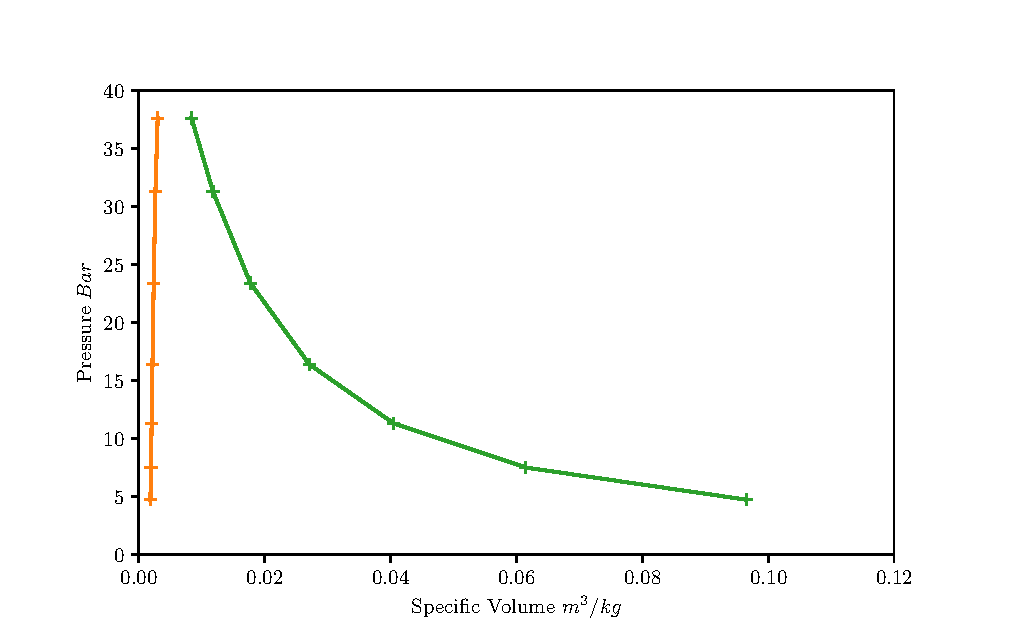
\includegraphics[width=\columnwidth]{fig2.eps}
    \end{figure}
\end{document}